Some words go here

\begin{figure}[htb]
	\centering
	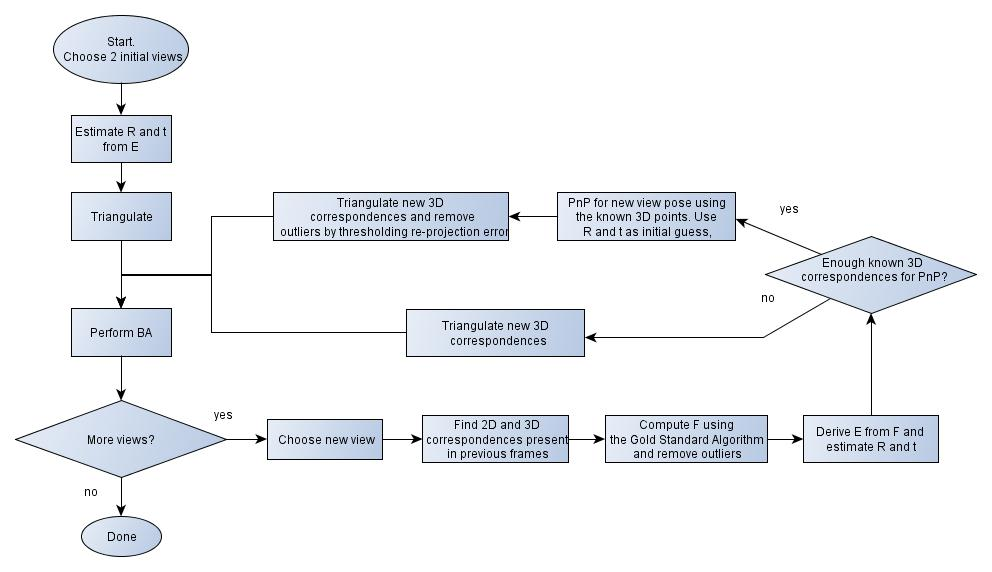
\includegraphics[width=160mm]{images/example1.jpg}
	\caption[This text ends up at the list of figures]{\textit{Data flow between modules.(example image)}}
	\label{fig:block_overview_fig}  %Skapar referens till figuren
\end{figure}


\subsection{Description}
The software part of the system will be the largest part, as all the processing and interfacing will be done in software.
The program will run as a cloud based service hosted on LIUs cloud.

All code will be written in C++ using the C++ 11 standard.

The software will be structured to be as modular as possible, with as small dependencies between modules as possible.

\subsection{External dependencies}
The software will be written using the OpenCV library to handle the image processing tasks.

Particular cameras may need specialized APIs, the system will be written in such a way that replacing the camera communication module is a simple as possible.

Some library to handle communication with LIUs REST API will also be needed.

Diagnostic and debugging tools will depend on the QT GUI framework.

To build the software from source code the cmake build system will be needed, aswell as a C++ 11 capable compiler.

\subsection{Compatibility}
The software will be possible to compile and run on alla major platforms (Windows/Linux/OS X). The system will expose and API that allows modules for arbitrary cameras to be written.

\subsection{Limitations}
Processing of image data must not require to 

\subsection{Software Requirements}
\label{sec:software_req}
\reqtable
{	
	\addreq{The system runs on Windows based plattforms}{1}
	\addreq{The system runs on Linux based plattforms}{1}
	\addreq{The system runs on OS x}
	\addreq{The system is modular with respect to the camera manufacturer and/or network API}{1}
}